\documentclass[main.tex]{subfiles}
\begin{document}

\section{The Klein paradox}

\marginpar{Thursday\\ 2020-3-19, \\ compiled \\ \today}

The fact that it was not possible to derive a conserved charge for the KG equation is not just a mathematical inconvenience: we will use a gedankenexperiment to show the physical consequences of this. 

Consider the scattering of a particle, which is described by a pure plane wave, on a an electromagnetic potential step.
Suppose we are in a frame in which \(qA^{\mu } = (V(x), \vec{0})\); if we are not in such a frame we can always perform a boost so that we are.
Also suppose that the potential looks like a step: \(V(x) = V_0 [x \geq 0]\). Here ``\(x\)'' refers to a 1d spatial coordinate. 

Now, suppose that we have an incoming wave with energy \(\omega \) and momentum \(k_{x}\) in the \(x<0\) region. 
Upon impact, there will in general be a reflected wave in the \(x<0\) region and a transmitted wave in the \(x>0\) region. We will call the former \(\varphi_{1}\) and the latter \(\varphi_{2}\). 

We can decompose both of these into a time and space exponential: \(\varphi_{i} (t, x) = e^{-i \omega t} \chi_{i}(x)\), for \(i = 1, 2\). 

Now, the incoming wave contributes to the global wavefunction with an exponential \(e^{ik_x x}\) in the \(x<0\) region. 
In the same region we can find the reflected wave, which has the opposite momentum; also, its amplitude is less than that of the incoming wave. We write its contribution to \(\chi_{1}\) as \(r e^{-i k_x x}\), where \(r\) is the reflection coefficient. 

By a similar reasoning, in the \(x>0\) region we will have a contribution \(t e^{i k_x^{\prime } x}\): the direction of propagation is the same as the incoming wave, the momentum might be different. In the end, our wavefunction looks like 
%
\begin{align}
\varphi (t, x) &= \varphi_1 [x\leq 0] + \varphi_2 [x \geq 0] \\
&= e^{-i \omega t} \qty[\chi_1 [x\leq 0] + \chi_2 [x \geq 0]] \\
&=
 e^{-i \omega t} \qty[ \qty(e^{i k_x x} + r e^{-i k_x x})[x\leq 0] + t e^{i k_x^{\prime }x } [x\geq 0]]
\,.
\end{align}

This wavefunction will need to satisfy the KG equation everywhere, however the equation has a different form in the two regions: if \(\DD^{\mu } = \partial^{\mu } + iqA^{\mu }\), then we can say that the two equations are 
%
\begin{align}
  \qty[\partial^{\mu } \partial_{\mu } + M^2] \varphi_1 &= 0 \\
  \qty[\DD^{\mu } \DD_{\mu } + M^2] \varphi_2 &= 0 
\,,
\end{align}
%
so we can insert the solutions into the equations: for the region without potential we get
%
\begin{align}
\qty[\partial^{\mu } \partial_{\mu } + M^2] \varphi_1 &= \qty[+ \partial_0^2 - \partial_{x}^2 + M^2 ] \qty[e^{-i \omega t} \qty(e^{ik_{x}x} + r e^{-ik_x x})]   \\
&= (-i\omega)^2 \varphi_1 + M^2 \varphi_1 - e^{-i \omega t}\partial_{x}^2  \qty(e^{ik_{x}x} + r e^{-ik_x x}) \\
&= -\omega^2 \varphi_1 + M^2 \varphi_1 - e^{-i \omega t}  \qty((ik_x)^2 e^{ik_{x}x} + r (-ik_x)^2 e^{-ik_x x}) \\
&= \qty[-\omega^2 + M^2 + k_x^2 ] \varphi_1  
\,,
\end{align}
%
notice that even though the function has components with momentum in either direction it still is an eigenfunction of the operator \(\square\)! 
For the other region we can use the fact we discussed earlier: with the minimal substitution, the momentum becomes \(p^{\mu } = i \partial^{\mu } \rightarrow i \DD^{\mu } = p^{\mu } - qA^{\mu }\), so in our case we will have \(p^{0} \rightarrow \omega_{k} - q A^{0} = \omega_{k} - V_0 \), while \(p^{i} \rightarrow \vec{k}'\), since \(\vec{A} = 0\). We can substitute the energy directly since the potential is constant, so there is no \(\partial_0 V_0 \) term. 
Then, the rest of the calculation is perfectly analogous, with \(k_{x}'\) instead of \(k_x\).

So, we have the two relations 
%
\begin{align} \label{eq:dispersion-relation-general}
- \omega_k^2 + k_x^2 + M^2 = 0
\qquad \text{and} \qquad
- \qty(\omega_{k} - V_0 )^2 + k_x^{\prime 2}  + M^2 = 0
\,.
\end{align}

We choose the solutions in which the wave is propagating towards increasing \(x\): so we get 
%
\begin{align}
k_x = \sqrt{\omega_{k}^2  - M^2} 
\qquad \text{and} \qquad
k_x^{\prime} = \sqrt{\qty(\omega_{k} - V_0)^2 - M^2}
\,.
\end{align}

Now we must make these consistent with each other, by imposing that at the border the function be \(\mathcal{C}^{1}\). 

Why do we fix only the first derivative? Probably something to do with the fact that the KG eq is second order, so we would need \(\square = \DD^{\mu } \DD_{\mu }\) at the boundary, which cannot be the case.

We can work with the spatial components \(\chi_{i}\), since the time evolution factors. So, for continuity we get that \(\chi_1 (0) = \chi_2 (0)\) implies:
%
\begin{align}
1+r = t
\,,
\end{align}
%
while for differentiability we get that \(\partial_{x} \chi_1(0) = \partial_{x} \chi_2 (0)\) implies:
%
\begin{align}
i k_x  - r i k_x = i t k_x'
\implies
\frac{k_x'}{k_x} = \frac{1- r}{t}
\,.
\end{align}

Now, what do we know of these variables? Well, from the dispersion relations if we fix the mass \(M\), the energy \(\omega \) and the potential \(V_0 \) we have \(k_x\) and  \(k_x^{\prime }\). 
Then, from the two equations we have found we can calculate \(r\) and \(t\); their expressions are exactly those found in the nonrelativistic case. Since \(1-r = 2-t\) we have 
%
\begin{align}
\frac{k_{x}'}{k_x} = \frac{2}{t} - 1 \implies 
\frac{k_x^{\prime } + k_x}{k_x} = \frac{2}{t}
\implies t = \frac{2 k_x}{k_x' + k_x}
\qquad \text{and} \qquad
r = t-1 = \frac{k_x - k_x'}{k_x' + k_x}
\,.
\end{align}

Now, we shall discuss the probability currents for the two regions: the formula is always 
%
\begin{align}
j^{\mu } = \frac{i}{2} \varphi^{*} \partial^{\mu } \varphi  + \frac{q}{2} A^{\mu } \varphi^{*} \varphi  + \text{c. c.}
\,,
\end{align}
%6
but in the first region the potential is identically zero. 

One non-obvious thing to consider is that, in general, we could have \(k_x'\) be either real or imaginary, since while \( \omega^2 - M^2\) must be \(>0\) there is no such constraint on \((\omega- V_0 )^2 - M^2\).
If we conjugate an exponential as \(\qty(e^{iz})^{*}\), the result is \(e^{-i z^{*}}\) for a general complex \(z\). 
The calculation is as follows:
%
\begin{align}
\rho_1 \overset{\text{def}}{=}  
j^{0}_{(1)} &= \frac{i}{2} e^{i \omega t} \partial^{0} e^{-i \omega t} \abs{\chi_1 }^2  + \text{c. c.} = \frac{2}{2} \omega \abs{\chi_1 }^2 
\marginnote{The \(\chi_1 \) is not time-dependent, we get two terms by adding the conjugate. We get a minus sign from lowering the index}  \\
j_1 \overset{\text{def}}{=} j^{x}_{(1)} &= - \frac{i}{2} \qty(e^{ik_x x} + r e^{-ik_x x}) \partial_{x} \qty(e^{ik_x x} + r e^{-ik_x x}) + \text{c. c. } \\
&= - \frac{2}{2} i (i k_x ) \qty(e^{ik_x x} + r e^{-ik_x x}) \qty(e^{ik_x x} - r e^{-ik_x x}) = k_x \qty(1 - \abs{r}^2)  \\
\rho_2 \overset{\text{def}}{=}  j^{0}_{(2)} &= \frac{i}{2} t^{*} e^{i \omega t} e^{-i k_x^{\prime *}x} t (-i \omega ) e^{-i \omega t} e^{i k_x^{\prime } x} + \frac{1}{2} V_0 \varphi^{*} \varphi  + \text{c. c.}  \\
&= (\omega - V_0 ) \abs{t}^2 e^{i \qty(k_x^{\prime }- k_x^{\prime *})x}  \\
j_2 \overset{\text{def}}{=} j^{x}_{(2)} &= -\frac{i}{2} t^{*} e^{i \omega t} e^{-i k_x^{\prime *} x} 
(i k_x^{\prime }) e^{-i \omega t} e^{i k_x^{\prime }x } + \text{c. c. }  \\
&= \frac{1}{2} \abs{t}^2 e^{i \qty(k_x^{\prime } - k_x^{\prime *})x} k_x^{\prime } + \text{c. c. }  \\
&= \frac{k_x^{\prime } + k_x^{\prime *}}{2} \abs{t}^2 e^{i \qty(k_x^{\prime } - k_x^{\prime *})x}
\,.
\end{align}

We can define the reflection and transmission coefficients, which are probabilities:
%
\begin{align}
\mathcal{R} = \frac{j _{\text{in}} - j_1}{j _{\text{in}}} = \abs{r}^2
\qquad \text{and} \qquad
\mathcal{T} = \frac{j_2}{j _{\text{in}}}
= \frac{k_x^{\prime } + k_x^{\prime *}}{2 k_x} \abs{t}^2 e^{i (k_x^{\prime } -k_x^{\prime *})x}
\,,
\end{align}
%
where \(j _{\text{in}} = k_x\). 
\todo[inline]{What is the motivation behind these definitions?}

Now, we have three possible cases for the behavior of \(k_x^{\prime }\): it is 
\begin{enumerate}
  \item real if \(\omega_{k} - M > V_0 \): this is the nonrelativistic case;
  \item imaginary if \(\abs{\omega_{k} - V_0 } < M\): this is the intermediate case;
  \item real again if \(\omega_{k} + M < V_0 \): this is the fully relativistic case.
\end{enumerate}

\begin{figure}[ht]
\centering
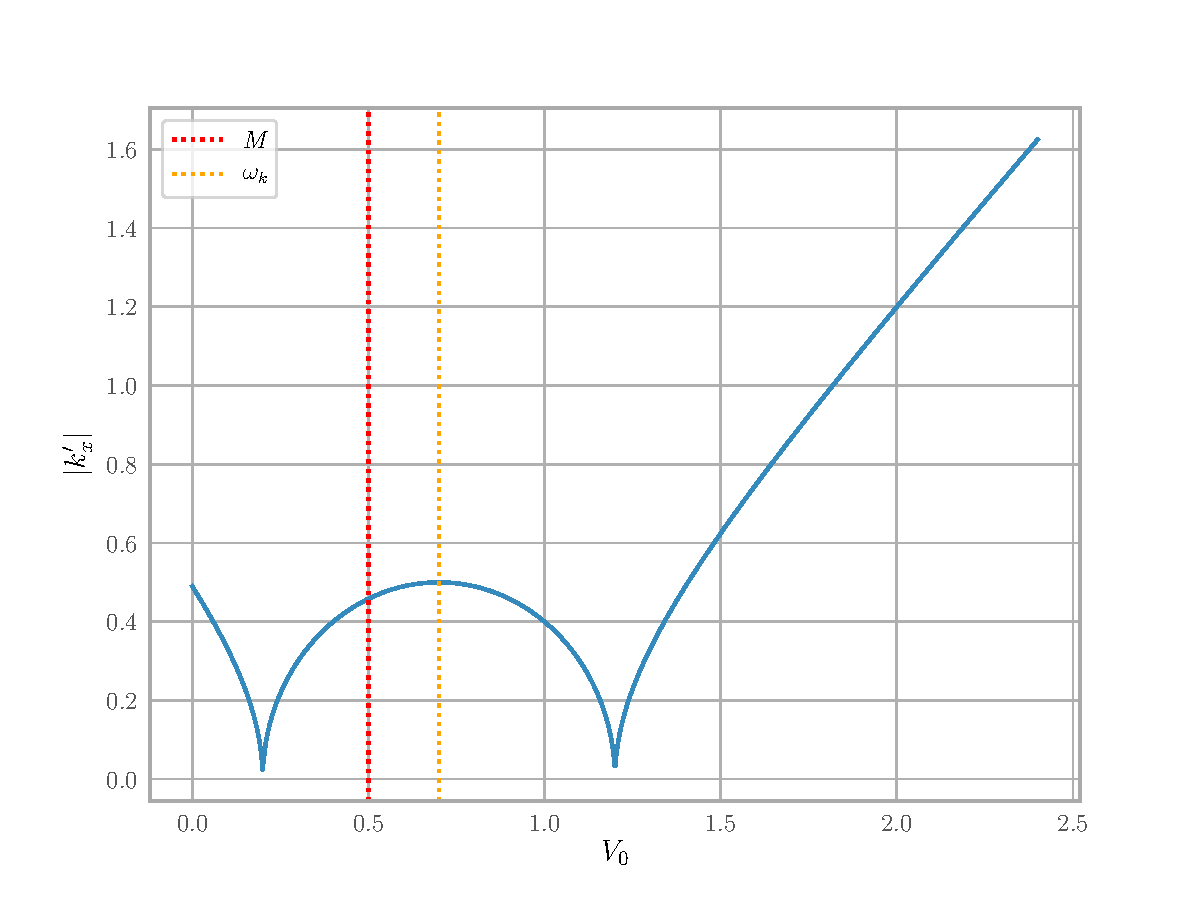
\includegraphics[width=\textwidth]{figures/primed_momentum_potential.pdf}
\caption{An illustration of how \(k_x^{\prime }\) changes as \(V_0 \) increases. We have fixed the mass \(M\) and the the energy \(\omega_{k}\) to \(\num{.5}\) and \(\num{.7}\) respectively. The regions are separated by the critical points of \(\abs{k_x'}\), at \(V_0 = \num{.2}\) and \(V_0 = \num{1.2}\) respectively. Do note that this is a plot of the \emph{absolute value} of \(k_x^{\prime }\): in the intermediate region it is purely imaginary.}
\label{fig:primed_momentum_potential}
\end{figure}

This is shown in figure \ref{fig:primed_momentum_potential}.
 
\todo[inline]{The professor states that the NR approximation can only be applied in the first case: however, vanilla QM can deal with the second case, as long as \(V_0 < \omega_{k}\).}

\subsubsection{Nonrelativistic case}

Now, \(k_x\) and \(k_x'\) are both real, so \(k_x^{\prime } = k_x^{\prime *}\), which means that the probability currents read: 
%
\begin{align}
\rho_1 &= \omega \abs{\chi_1 }^2
&
j_1 &= k_x \qty(1 - \abs{r}^2) \\
\rho_2 &= (\omega - V_0 ) \abs{t}^2 
&
j_2 &=  k_x^{\prime } \abs{t}^2 
\,,
\end{align}
%
and, since \(r\) and \(r\) are both (real and) \(<1\) these quantities are all positive. Also, we must have \(k_x' < k_x\), so the quantities 
%
\begin{align}
\mathcal{R} &= \abs{r}^2
\qquad \text{and} \qquad
\mathcal{T} = \frac{k_x'}{k_x} \abs{t}^2
\,
\end{align}
%
are both \(<1\). So, it will be consistent if we impose (?) a probabilistic Born-like interpretation in which these coefficients are reflection and transmission probabilities, with \(\mathcal{R} + \mathcal{T} = 1\).

\subsubsection{Intermediate case}

Now, we have \(\abs{\omega_{k} - V_0 } < M\), so, while \(k_x>0\), 
%
\begin{align}
k_x' = \pm i \sqrt{M^2 - \qty(\omega_{k} - V_0 )^2}
\,.
\end{align}

\todo[inline]{In principle we could have both \(+\) or \(-\), right? Do we select \(+i\) by normalization later?}

Now, in our computation of the probability density \(\rho_2 \) we will have a factor 
%
\begin{align}
\exp(i (k_x' - k_x^{\prime *})x) = \exp(\pm 2 i^2 \abs{k_x'}x) =  \exp(\mp 2 \abs{k_x^{\prime }} x)
\,,
\end{align}
%
while for the probability current \(j_2 \) we will get a factor \(k_x^{\prime } + k_x^{\prime *} = 0 \) multiplying everything.

\todo[inline]{The solution with \(\exp(+ 2\abs{k_x'} x)\) is unphysical (not normalizable), so we discard it (?)}

So, in the end we get 
%
\begin{align}
\rho_1 &= \omega \abs{\chi_1 }^2
&
j_1 &= k_x \qty(1 - \abs{r}^2) \\
\rho_2 &= (\omega - V_0 ) \abs{t}^2 e^{-2 \abs{k_x^{\prime }} x}
&
j_2 &= 0 
\,.
\end{align}

Notice that in the intermediate region we can have both \(V_0 < \omega_{k}\) and \(V_0 > \omega_{k}\). 

In this case, we get for the reflection and transmission probabilities 
%
\begin{align}
\mathcal{R} = \abs{r}^2 = \abs{\frac{k_x - i k_x^{\prime }}{k_x + i k_x^{\prime }}} = \abs{\frac{z}{z^{*}}}^2 = 1
\marginnote{The ratio of \(z\) and \(z^{*}\) is only a phase}
\,,
\end{align}
%
while \(\mathcal{T} \propto j_2 = 0\). 

So, in this case the particle is certainly reflected; this is compatible with the probabilistic interpretation \(\mathcal{R} + \mathcal{T} = 1\). 
However, \(\rho_2  \) is not positive defined so it cannot be interpreted as a probability density in general. 

If \(V_0 < \omega_{k} \) we still get the vanilla-QM result of \(\rho_2 \sim e^{-2 \abs{k_x^{\prime }}x}\): the particle penetrates the classically forbidden region. 
This effect is suppressed as \(V_0 \) increases. 

\subsubsection{Fully relativistic case}

This is the situation which is completely outside the realm of classical QM description, in which we expect to see relativistic effects. 
We have \(V_0 > \omega_{k} + M \). 

Now 
%
\begin{align}
k_x^{\prime } = \pm \sqrt{(\omega_{k} - V_0 )^2 - M^2} \in \mathbb{R}
\,,
\end{align}
%
so the densities are 
%
\begin{align}
\rho_1 &= \omega \abs{\chi_1 }^2
&
j_1 &= k_x \qty(1 - \abs{r}^2) \\
\rho_2 &= (\omega - V_0 ) \abs{t}^2 < 0 
&
j_2 &= k_{x}^{\prime } \abs{t}^2 
\,,
\end{align}
%
where the sign of \(j_2 \) is determined by that of \(k_x^{\prime }\), which is not necessarily positive. 
Actually, it must be negative: to see this, we can calculate the group velocity, which would be the global velocity of the wavepacket we are approximating. We can calculate \(\omega_{k}\) from the dispersion relation \eqref{eq:dispersion-relation-general} to get
%
\begin{align}
v_G = \pdv{\omega_{k} }{k_x^{\prime }} 
= \pdv{k_x^{\prime }} \qty(V_0 + \sqrt{k_x^{\prime 2} + M^2})
= \frac{k_x^{\prime }}{\sqrt{k_x^{\prime 2} + M^2}}
= \frac{k_x^{\prime }}{\omega_{k} - V_0 }
\,,
\end{align}
%
where we used the dispersion relation again in the last step. 
Now, for the packet to propagate forward we need \(v_G > 0\), but since the denominator is negative this means \(k_x^{\prime } < 0\). 

Then, we will have 
%
\begin{align}
r = \frac{k_x - k_x^{\prime }}{k_x + k_x^{\prime }} 
\implies 
\mathcal{R} = \abs{\frac{k_x - k_x^{\prime }}{k_x + k_x^{\prime }}}^2 > 1
\,,
\end{align}
%
while the other coefficient is 
%
\begin{align}
\mathcal{T} = \frac{k_x^{\prime }}{k_x} \abs{t}^2  
= \frac{k_x^{\prime }}{k_x} \abs{\frac{2 k_x}{k_x^{\prime } + k_x}}^2 
= k_x^{\prime } \frac{4 k_x}{(k_x^{\prime } + k_x)^2}
< 0
\,.
\end{align}
%

So, we can still maintain the condition \(\mathcal{R} + \mathcal{T} =1\), but reflection is ``more than certain''? Surely this is not the correct physical interpretation. 

This is the heart of the Klein-Gordon paradox. 

What is actually happening is that in our description we are fixing the number of particles to be one; a proper (``grand-canonical'' instead of ``canonical'', in statistical mechanics terms) description of the situation would allow us to see that the energy in the system is enough to create real particle-antiparticle pairs.

The antiparticles gain energy under the potential (since they perceive it as \(-V_0 \), having a negative charge), so they are transmitted, while the particles are reflected. On average, then, more than one particle is reflected. 

In order to properly study these extreme conditions, we need the new paradigm of \emph{Quantum Field Theory}. 

\end{document}